\documentclass{article}%
\usepackage[T1]{fontenc}%
\usepackage[utf8]{inputenc}%
\usepackage{lmodern}%
\usepackage{textcomp}%
\usepackage{lastpage}%
\usepackage{authblk}%
\usepackage{graphicx}%
%
\title{Inhibition of rhabdomyosarcoma cell and tumor growth by targeting specificity protein (Sp) transcription factors}%
\author{Jordan Khan}%
\affil{Discipline of Microbiology and Immunology, School of Molecular and Biomedical Science, University of Adelaide, Adelaide, Australia}%
\date{01{-}01{-}2013}%
%
\begin{document}%
\normalsize%
\maketitle%
\section{Abstract}%
\label{sec:Abstract}%
A recent study by scientists at Harvard Medical School finds that disrupting the sleep{-}wake cycle in animals with low levels of melatonin disrupts its biological activity as an indicator of circadian rhythm in the body. The findings have been published in the journal Nature Methods.\newline%
Certain chemicals and steroid hormone stimulation have been shown to correlate with obesity in animals without eating processed foods. Research has also been conducted to determine whether a local biochemical response in cells is also related to weight gain. These results were not observed in mammals.\newline%
Dr. Kevin Coonarman, a member of the Harvard Medical School and Chief of the Office of Kinesiology and the Head of the Experimental Weight Loss Programs, published the research in Nature Methods.\newline%
The study employed mouse models of Parkinsons disease and diabetes to test the effects of a local and local{-}regulate micro{-}environmental process known as circadian oscillation, which is a mechanism at the center of the human circadian system. The concentrations of circadian biological activities in the circadian system are not known to be locally inconsistent with body weight; this creates an atlas of the circadian oscillations in the mice which show an association with alterations in metabolism and diet.\newline%
The good news is that exposure to a well{-}established sleep{-}wake condition  disrupted melatonin production  in the early stages of Parkinsons disease resulted in overweight rats with elevated concentrations of metabolically normal{-}level metabolites which persisted in both the control and control rat groups of the study. The bad news is that exposing the rats to a disrupted diet in the middle of the brain region was associated with a significantly higher concentration of glucose at the nucleus autodilation imager.

%
\subsection{Image Analysis}%
\label{subsec:ImageAnalysis}%


\begin{figure}[h!]%
\centering%
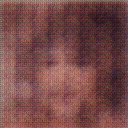
\includegraphics[width=150px]{500_fake_images/samples_5_13.png}%
\caption{A Black And White Photo Of A Black And White Cat}%
\end{figure}

%
\end{document}